\begin{frame}[parent={ie:agenda}, hasnext=true, hasprev=false]
	\frametitle{ISO 9126}

	\begin{block:concept}{ISO 9126}
		Conjunto de normas ISO/IEC sobre a qualidade de produto de software.
	\end{block:concept}
	
	\begin{block:fact}{Partes da norma}
		\begin{itemize}
			\item ISO/IEC 9126-1: Modelo de qualidade.
			\item ISO/IEC 9126-2: Métricas externas.
			\item ISO/IEC 9126-3: Métricas internas.
			\item ISO/IEC 9126-4: Métricas de qualidade em uso.
		\end{itemize}
	\end{block:fact}

	\begin{block:fact}{AVISO}
		A coleção de norma ISO 9126 foi aposentada/substituída pela coleção
		da ISO 25000!
	\end{block:fact}
	
	\note{
		\begin{itemize}
			\item Primeiros esforços para padronização: 1978
			\item Início de desenvolvimento da norma: 1985
			\begin{itemize}
				\item Information Technology -- Software product evaluation -- Quality
				characteristics and guidelines for their use
			\end{itemize}
			\item Publicada em 1991
			\item Atualizada em 2001
			\begin{itemize}
				\item Software Engineering -- Product Quality
			\end{itemize}
			\item ``Aposentada'' em 2008 pela ISO 25000
		\end{itemize}
	}
\end{frame}


\begin{frame}[hasnext=false, hasprev=true]
	\frametitle{ISO 9126}
	\framesubtitle{ISO 9126-1: Modelo de qualidade}
	
	\begin{block:fact}{Modelo de qualidade}
		Organizada em características, subcaracterísticas e métricas.
	\end{block:fact}
	
	\begin{block:fact}{}
		Modelo organizado hierarquicamente por características e subcaracterísticas.
		\begin{itemize}
			\item 6 características
			\item 27 subcaracterísticas
			\item ao menos uma métrica por característica
		\end{itemize}
	\end{block:fact}
\end{frame}


\begin{frame}
	\frametitle{ISO 9126-1: Modelo de qualidade}
	\framesubtitle{Características}
	
	\begin{block:fact}{Características}
		\begin{itemize}
			\item Funcionalidade
			\item Confiabilidade
			\item Usabilidade
			\item Eficiência
			\item Manutenibilidade
			\item Portabilidade
		\end{itemize}
	\end{block:fact}

	\begin{block:fact}{}
		\begin{itemize}
			\item \textbf{O que?} Funcionalidade
			\item \textbf{Quando e como?} Confiabilidade, usabilidade, eficiência,
			manutenibilidade e portabilidade.
		\end{itemize}
	\end{block:fact}
\end{frame}


\begin{frame}
	\frametitle{ISO 9126-1: Modelo de qualidade}
	\framesubtitle{Características}
	
	\begin{block:fact}{Funcionalidade}
		Conjunto de atributos que evidenciam a existência de um conjunto de funções
		e suas propriedades especificadas.

		Funções: aquilo que satisfaz as necessidades implícitas e explícitas
		(requisitos funcionais)
	\end{block:fact}
	
	\begin{block:fact}{Subcaracterísticas}
		\begin{itemize}
			\item Adequação: propõe-se a fazer o que é apropriado?
			\item Acurácia: faz o que foi proposto de forma correta?
			\item Interoperabilidade: é capaz de interagir com os sistemas especificados?
			\item Segurança de acesso: evita acesso não autorizado a programas e dados?
			\item Conformidade: está de acordo com normas técnicas e aspectos legais
			relacionados à funcionalidade?
		\end{itemize}
	\end{block:fact}
\end{frame}



\begin{frame}
	\frametitle{ISO 9126-1: Modelo de qualidade}
	\framesubtitle{Características}
	
	\begin{block:fact}{Confiabilidade}
		Conjunto de atributos que evidenciam a capacidade do software manter seu nível
		de desempenho sob condições estabelecidas durante um período de tempo
		estabelecido.
	\end{block:fact}
	
	\begin{block:fact}{Subcaracterísticas}
		\begin{itemize}
			\item Maturidade: com que frequência apresenta defeitos?
			\item Tolerância a falhas: Na ocorrência de um erro, como o sistema
			reage? Ocorre uma falha?
			\item Recuperabilidade: O produto é capaz de se recuperar em casos de
			falhas?
			\item Conformidade
		\end{itemize}
	\end{block:fact}
\end{frame}



\begin{frame}
	\frametitle{ISO 9126-1: Modelo de qualidade}
	\framesubtitle{Características}
	
	\begin{block:fact}{Usabilidade}
		Conjunto de atributos que evidenciam o esforço necessário para utilizar o
		software bem como para o julgamento individual deste uso.
	\end{block:fact}
	
	\begin{block:fact}{Subcaracterísticas}
		\begin{itemize}
			\item Inteligibidade: É fácil entender o conceito da aplicação e sua
			aplicabilidade?
			\item Apreensibilidade: É fácil aprender a usar?
			\item Operabilidade: É fácil de operar e controlar?
			\item Atratividade: É atrativa ao usuário?
			\item Conformidade
		\end{itemize}
	\end{block:fact}
\end{frame}


\begin{frame}
	\frametitle{ISO 9126-1: Modelo de qualidade}
	\framesubtitle{Características}
	
	\begin{block:fact}{Eficiência}
		Conjunto de atributos que evidenciam o relacionamento entre o nível de
		desempenho do software e quantidade de recursos usados sob condições
		previamente estabelecidas.
	\end{block:fact}
	
	\begin{block:fact}{Subcaracterísticas}
		\begin{itemize}
			\item Comportamento em relação ao tempo
			\item Comportamento em relação aos custos
			\item Conformidade
		\end{itemize}
	\end{block:fact}
\end{frame}


\begin{frame}
	\frametitle{ISO 9126-1: Modelo de qualidade}
	\framesubtitle{Características}
	
	\begin{block:fact}{Manutenibilidade}
		Conjunto de atributos que evidenciam o esforço necessário para fazer
		modificações no software.
	\end{block:fact}
	
	\begin{block:fact}{Subcaracterísticas}
		\begin{itemize}
			\item Analisabilidade: é fácil encontrar um defeito quando detectada uma falha?
			\item Modificabilidade: É fácil modificar e adaptar o software?
			\item Estabilidade: Existe risco de efeitos inesperados quando realizadas alterações?
			\item Testabilidade: É fácil validar o software modificado?
			\item Conformidade
		\end{itemize}
	\end{block:fact}
\end{frame}


\begin{frame}
	\frametitle{ISO 9126-1: Modelo de qualidade}
	\framesubtitle{Características}
	
	\begin{block:fact}{Portabilidade}
		Conjunto de atributos que evidenciam a capacidade do software ser transferido
		de um ambiente para outro.
	\end{block:fact}
	
	\begin{block:fact}{Subcaracterísticas}
		\begin{itemize}
			\item Adaptabilidade: É fácil adaptar para ambientes diferentes?
			\item Instalação: É fácil de instalar?
			\item Capacidade de ser substituído: É fácil substituir este software por outro?
			\item Coexistência: Pode coexistir com outros produtos e compartilhar os recursos?
			\item Conformidade
		\end{itemize}
	\end{block:fact}
\end{frame}


\begin{frame}
	\frametitle{ISO 9126-1: Modelo de qualidade}
	\framesubtitle{Métricas internas e externas}
	
	\begin{block:fact}{Subcaracterísticas e métricas}
		Subcaracterísticas são medidas por métricas internas e externas.
		\begin{itemize}
			 \item Métricas externas: exemplificadas na ISO/IEC 9126-2
			 \item Métricas internas: exemplificadas na ISO/IEC 9126-3
		\end{itemize}
	\end{block:fact}
	
	\begin{block:concept}{Métrica interna}
	Aplicável aos artefatos de software (durante o desenvolvimento)
	\end{block:concept}

	\begin{block:concept}{Métrica externa}
	Aplicável ao produto de software durante a fase de teste (aplicada pelo
	desenvolvedor, mas com o ponto de vista do usuário)
	\end{block:concept}
\end{frame}



\begin{frame}
	\frametitle{ISO 9126}
	\framesubtitle{Qualidade em uso}
	
	\begin{block:fact}{Qualidade em uso}
		Refere-se ao uso do software em ambiente específico e não às propriedades
		do software.
	\end{block:fact}
\end{frame}


\begin{frame}
	\frametitle{ISO 9126}
	\framesubtitle{Qualidade em uso}
	
	\begin{block:fact}{Características}
		\begin{itemize}
			\item Eficácia
			\begin{itemize}
				\item Permite que o usuário atinja metas com acurácia e completitude
			\end{itemize}
			
			\item Produtividade
			\begin{itemize}
				\item Permite que o usuário utilize quantidade apropriada de recursos
			\end{itemize}

			\item Segurança
			\begin{itemize}
				\item Apresentar níveis aceitáveis de risco a pessoas, negócio, propriedade e ambiente
			\end{itemize}

			\item Satisfação
			\begin{itemize}
				\item Satisfaz o usuário
			\end{itemize}
		\end{itemize}
	\end{block:fact}
\end{frame}

\begin{frame}
	\frametitle{ISO 9126}
	\framesubtitle{Qualidade em uso}
	
	\begin{block:fact}{Métricas}
		Exemplificadas na ISO/IEC 9126-4.
	\end{block:fact}
\end{frame}


\begin{frame}
	\frametitle{ISO 9126}
	\framesubtitle{Limitações}
	
	\begin{block:fact}{Limitações}
		\begin{itemize}
			\item Falta de evidências para a criação da norma
			\begin{itemize}
				\item Não foram executados estudos experimentais para avaliar as
				características e subcaracterísticas
			\end{itemize}
			
			\item Difícil aplicação
			\begin{itemize}
				\item Falta de diretivas (\foreign{guidelines})
				\item ``Genérica demais''
			\end{itemize}
		\end{itemize}
	\end{block:fact}
\end{frame}

\begin{frame}
	\frametitle{ISO 9126}
	\framesubtitle{Limitações}
	
	\begin{block:fact}{Measuring software product quality: a survey of ISO/IEC 9126 (Jung et al.)}
		\begin{itemize}
			\item Qualidade é um vetor (dimensões são as características de qualidade).

			\item Fatores analisados: todos menos as características de confiabilidade
			e todas as subcaracterísticas sobre conformidade.
			
			\item Cada questionário avaliou o mesmo produto quanto às subcaracterísticas
			da norma.
			
			\item PCA para identificar se os fatores realmente caracterizam uma
			dimensão (correlação entre as subcaracterísticas quanto à qualidade do
			produto).
		\end{itemize}
	\end{block:fact}
\end{frame}


\begin{frame}
	\frametitle{ISO 9126}
	\framesubtitle{Limitações}
	
	\begin{block:fact}{Measuring software product quality: a survey of ISO/IEC 9126 (Jung et al.)}
		\centering
		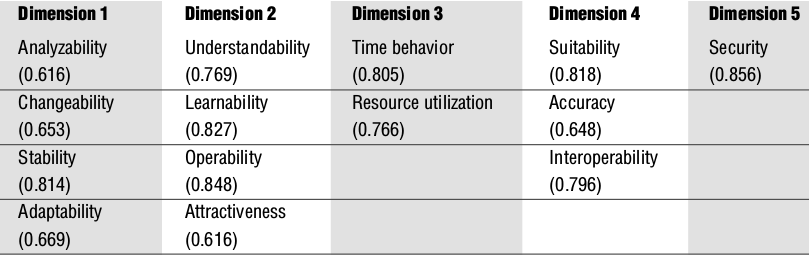
\includegraphics[width=\textwidth]{software-engineering/project-management/product/iso9126/jung-etal}
	\end{block:fact}
	
	\note{
		\begin{itemize}
			\item Quatro subcaracterísticas não estão presentes (correlação inferior a
			0,6): testabilidade, instalabilidade, substituibilidade, coexistência)
			
			\item Primeira dimensão não é consistente (adaptabilidade)
			
			\item Segurança não está correlacionada com outras características
		\end{itemize}
	}
\end{frame}

%
%
%\begin{frame}
%	\frametitle{ISO 9126}
%	\framesubtitle{Limitações}
%	
%	\begin{block:fact}{The use and usefulness of the ISO/IEC 9126 quality standard (Al-Kilidar et al.)}
%		\begin{itemize}
%			\item Avaliação de produto com a ISO/IEC 9126 por alunos de graduação
%			\begin{itemize}
%				\item Avaliação do projeto (design) de um produto
%			\end{itemize}
%			
%			\item Conclusão: norma é inútil
%		\end{itemize}
%	\end{block:fact}
%\end{frame}
%
%
%\begin{frame}
%	\frametitle{ISO 9126}
%	\framesubtitle{Limitações}
%	
%	\begin{block:fact}{The use and usefulness of the ISO/IEC 9126 quality standard (Al-Kilidar et al.)}
%		Limitações do estudo:
%		\begin{itemize}
%			\item Avaliaram artefato ``design'', não o produto
%			\item Não utilizaram um processo de avaliação
%			\begin{itemize}
%				\item Não definiram métricas (norma apenas \textbf{sugere} métricas)
%				\item Não treinaram avaliações antes de executar o experimento
%			\end{itemize}
%		\end{itemize}
%	\end{block:fact}
%\end{frame}
%
%
%\begin{frame}
%	\frametitle{ISO 9126}
%	\framesubtitle{Limitações}
%	
%	\begin{block:fact}{The use and usefulness of the ISO/IEC 9126 quality standard (Al-Kilidar et al.)}
%		Resultados úteis do estudo:
%		\begin{itemize}
%			\item Norma realmente possui problemas quanto a definições de termos
%			
%			\item Hierarquização das características/subcaracterísticas e seleção de
%			métricas
%			\begin{itemize}
%				\item Métrica útil para mais de uma subcaracterística
%				\item Isso não é vedado pela norma, mas ela passa a impressão de que sim
%			\end{itemize}
%			
%			\item Não são especificados requisitos para os dados coletados
%		\end{itemize}
%	\end{block:fact}
%\end{frame}